%%%%%%%%%%%%%%%%%%%%%%%%%%%%%%%%%%%%%%%%%%%%%%%%%%%
\documentclass[envcountsame,envcountchap]{svmono}

% scegliere le opzioni per []  come richiesto dalla lista 
% nella Reference Guide, Sez. 2.2

\usepackage{makeidx}         % permette di generare l'indice
\usepackage{graphicx}        % pacchetto grafico standard LaTeX 
                             % per l'inclusione di file immagine
\graphicspath{{./}{Figure/}}
\usepackage{multicol}        % usato per l'indice a due colonne
\usepackage[bottom]{footmisc}% mette le note a pie' di pagina
\usepackage[italian]{babel}
% etc.
% si veda la lista di ulteriori pacchetti utili 
% nella Reference Guide, Sez. 2.3, 3.1-3.3

\def\theoremname{Teorema}
\makeindex             % usato per l'indice degli argomenti 
                       % si prega di usare lo stile svind.ist con 
                       % il vostro programma makeindex


%%%%%%%%%%%%%%%%%%%%%%%%%%%%%%%%%%%%%%%%%%%%%%%%%%%%%%%%%%%%%%%%%%%%%

\begin{document}

\author{Prof. Giovanni Viterbo \\ Andrea Lops}
\title{Lezioni di Geometria e Algebra}
\subtitle{-- Raccolta di dispense --}
\date{Luglio 2020 versione 0.2.4}
\maketitle

\frontmatter%%%%%%%%%%%%%%%%%%%%%%%%%%%%%%%%%%%%%%%%%%%%%%%%%%%%%%

%%%%%%%%%%%%%%%%%%%%%%% dedic.tex %%%%%%%%%%%%%%%%%%%%%%%%%%%%%%%%%
%
% Esempio di dedica
%
% Usare questo file come template per il vostro documento.
%
%%%%%%%%%%%%%%%%%%%%%%%% Springer-Verlag %%%%%%%%%%%%%%%%%%%%%%%%%%

\thispagestyle{empty}
\vspace*{3.5cm}
\begin{flushright}

% scrivere qui
{\large La vostra dedica va qui}

\end{flushright}




%%%%%%%%%%%%%%%%%%%%%% pref_it.tex %%%%%%%%%%%%%%%%%%%%%%%%%%%%%%%%%%%%%
%
% Esempio di prefazione
%
% Usare questo file come template per il vostro documento.
%
%%%%%%%%%%%%%%%%%%%%%%%% Springer-Verlag %%%%%%%%%%%%%%%%%%%%%%%%%%

\preface

%% Scrivere qui la prefazione
Ecco le parole d'oro


%% Si prega di  "firmare" la prefazione
\vspace{1cm}
\begin{flushright}\noindent
Localit\`{a},\hfill {\it Nome Cognome}\\
mese anno\hfill {\it Nome Cognome}\\
\end{flushright}




\tableofcontents


\mainmatter%%%%%%%%%%%%%%%%%%%%%%%%%%%%%%%%%%%%%%%%%%%%%%%%%%%%%%%
%%%%%%%%%%%%%%%%%%%%%%%% part.tex %%%%%%%%%%%%%%%%%%%%%%%%%%%%%%%%%%
%
% esempio di titolo della parte
%
% Usare questo file come template per il vostro documento.
%
%%%%%%%%%%%%%%%%%%%%%%%% Springer-Verlag %%%%%%%%%%%%%%%%%%%%%%%%%%


\part{Titolo della parte}

%%%%%%%%%%%%%%%%%%%%% chapter.tex %%%%%%%%%%%%%%%%%%%%%%%%%%%%%%%%%
%
% esempio di capitolo
%
% Usare questo  file come template per il vostro documento.
%
%%%%%%%%%%%%%%%%%%%%%%%% Springer-Verlag %%%%%%%%%%%%%%%%%%%%%%%%%%

\chapter{Titolo del capitolo}
\label{intro} % Fornire sempre un'unica label
% usare \chaptermark{}
% per alterare o aggiustare l'intestazione del capitolo nella running head

Il vostro testo va qui.  Suddividere il testo in paragrafi  con i comandi 
 standard di \LaTeX\ .

\section{Titolo di primo livello}
\label{sec:1}
% Fornire sempre un'unica label
% ed usare \ref{<label>} per i riferimenti (cross-references)
% e \cite{<label>} per le citazioni bibliografiche
% usare \sectionmark{}
% per alterare o aggiustare l'intestazione della sezione nella  running head
Il vostro testo va qui. Usare  i comandi standard di  \LaTeX\ per le citazioni e i riferimenti bibliografici
\cite{monograph}.

\subsection{Titolo di secondo livello}
\label{sec:2}
Il vostro testo va qui.

\begin{equation}
\vec{a}\times\vec{b}=\vec{c}
\end{equation}

\subsubsection{Titolo di terzo livello}
Il vostro testo va qui. % Usare l'automatismo \LaTeX\ per i riferimenti e per le citazioni, si veda la Sez.~\ref{sec:1}.

\paragraph{Titolo del paragrafo} %
Il vostro testo va qui.

\subparagraph{Titolo del sotto-paragrafo.} Il vostro testo va qui.%
%
\index{paragrafo}
% Usare il comando \index{} per inserire le proprie parole chiave
%
% Per le tabelle usare
%
\begin{table}
\centering
\caption{Scrivere qui la didascalia della tabella}
\label{tab:1}       % Fornire una label unica
%
% Per le tabelle LaTeX usare
%
\begin{tabular}{lll}
\hline\noalign{\smallskip}
prima & seconda & terza  \\
\noalign{\smallskip}\hline\noalign{\smallskip}
numero & numero & numero \\
numero & numero & numero \\
\noalign{\smallskip}\hline
\end{tabular}
\end{table}
%
%
% Per le figure usare
%
\begin{figure}
\centering
% Usare il comando appropriato per il vostro programma di inserzione dell figure
% per inserire il file immagine.
% Ad esempio, con l'opzione graphics usare
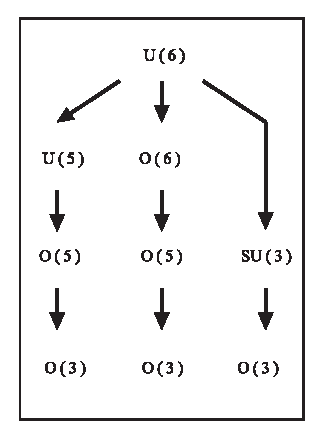
\includegraphics[height=4cm]{figure.eps}
%
% Altrimenti, usare
%\picplace{5cm}{2cm} % Fornire la corretta altezza e larghezza in cm
%
\caption{Scrivere qui la didascalia della figura}
\label{fig:1}       % Fornire una label unica
\end{figure}
%
% Per environments integrati usare
%
\begin{theorem}
Qui il testo del teorema.
\end{theorem}
%
% oppure
%
\begin{lemma}
Qui il testo del lemma.
\end{lemma}
%
%
% Problemi o Esercizi dovrebbero essere ordinati per capitolo
\section*{Problemi}
\addcontentsline{toc}{section}{Problemi}
%
% Use the following environment.
% Don't forget to label each problem;
% the label is needed for the solutions' environment
\begin{prob}
\label{prob1}
Il problema\footnote{Nota a pi\`{e} pagina} \`{e} descritto qui. Il problema \`{e} descritto qui. Il problema \`{e} descritto qui. \end{prob}

\begin{prob}
\label{prob2}
\textbf{Titolo del problema}\\
(a) La prima parte del problema \`{e} descritta qui.\\
(b) La seconda parte del problema \`{e} descritta qui.
\end{prob}



%

%\include{chapter}
%\appendix
%\include{appendix}

\backmatter%%%%%%%%%%%%%%%%%%%%%%%%%%%%%%%%%%%%%%%%%%%%%%%%%%%%%%%
\chapter*{Soluzioni}
\addcontentsline{toc}{chapter}{Soluzioni}
\markboth{Soluzioni}{Soluzioni}

\section*{Problemi del capitolo~\ref{intro}}

\begin{sol}{prob1}
La soluzione \`{e} presentata qui.
\end{sol}


\begin{sol}{prob2}
\textbf{Titolo del problema}\\
(a) La soluzione della prima parte del problema  \`{e} presentata qui.\\
(b) La soluzione della seconda parte del problema  \`{e} presentata qui.
\end{sol}


%%%%%%%%%%%%%%%%%%%%%%%% referenc_it.tex %%%%%%%%%%%%%%%%%%%%%%%%%%%%%%
% Esempio di referenze
%
%
% Usare questo file come template per il vostro documento.
%
%%%%%%%%%%%%%%%%%%%%%%%% Springer-Verlag %%%%%%%%%%%%%%%%%%%%%%%%%%

%
% Utenti BibTeX: usare
% \bibliographystyle{}
% \bibliography{}
%
% Non-utenti BibTeX: usare
\begin{thebibliography}{[KLR73]}
%
% ed usare \bibitem per creare referenze.
%
% Usare la sintassi ed il markup seguenti per le vostre referenze.
%
% Monografie
\bibitem[KLR73]{monograph} Kagan, A.M., Linnik, Y.V., Rao, C.R.:
Characterization Problems in Mathematical Statistics. Wiley, New York (1973)

% Contributed Works
\bibitem[Mey89]{contribution} Meyer, P.A.: A short presentation of
stochastic calculus. In: Emery, M. (ed) Stochastic Calculus in
Manifolds. Springer, Berlin Heidelberg New York (1989)

% Journal
\bibitem[MR97]{journal} Miller, B.M., Runggaldier, W.J.: Kalman
filtering for linear systems with coefficients driven by a hidden Markov
jump process. Syst. Control Lett., \textbf{31}, 93--102 (1997)

% Tesi
\bibitem[Ros77]{thesis} Ross, D.W.: Lysosomes and storage diseases. MA
Thesis, Columbia University, New York (1977)

\end{thebibliography}

\printindex

%%%%%%%%%%%%%%%%%%%%%%%%%%%%%%%%%%%%%%%%%%%%%%%%%%%%%%%%%%%%%%%%%%%%%%

\end{document}





